\section{Two Approaches}
There are two approaches to solve minimization problems.
\begin{enumerate}
	\item The \textit{classical} approach, also known as the \textit{indirect method}. The idea is to determine and characterize critical points of the functional $I$ with the help of necessary and sufficient conditions (something like ``$I'(u_*)=0$'' and ``$I''(u_*)\geq0$''). For that we need a suitable notion of derivative. Directional derivatives of $I$ are called \textit{variations}.\\

	However, there is a problem with the method. The existence of critical points is not clear. We will see that checking necessary conditions very often leads to solving a partial differential equation. Many examples are related to physics where we expect the existence of minimizers from our intuition, but this is no mathematical argument.
	\item The \textit{modern} approach, also known as the \textit{direct method}. Here the idea is to give sufficient conditions for the existence of minimizers. The general idea follows the steps:
	\begin{enumerate}
		\item Show that $I$ is bounded from below, i.e. $\inf_{u\in M}{I(u)}>-\infty$. Then choose an infimizing sequence $(u_k)_{k\in\mathbb{N}}\subset M$ with $I(u_k)\to\inf_{u\in M}{I(u)}$.
		\item Show that there exists a subsequence $(u_{k_\ell})_{\ell\in\mathbb{N}}$ of $(u_k)_{k\in\mathbb{N}}$ which converges in some sense to some $u_*\in M$.
		\item Show $\liminf_{\ell\to\infty}{I(u_{k_\ell})}\geq I(u_*)$. Then $u_*$ is a minimizer of $I$.
	\end{enumerate}
	We are talking about convergence, but what is the right topology? Strong, weak or weak* convergence? Choosing the right one is the mathematical challenge here! Verifying step (b) is easier in courser topologies, while (c) is easier in finer topologies. To see this, let $\tau_1,\tau_2$ be topologies on $X$, where $\tau_1$ is finer than $\tau_2$. Then $u_k\overset{\tau_1}{\to}u$ implies $u_k\overset{\tau_2}{\to}u$. On the other hand, if $I(u_k)\to I(u)$ for $u_k\overset{\tau_2}{\to}u$ then it also holds $I(u_k)\to I(u)$ if $u_k\overset{\tau_1}{\to}u$.\\[11pt]
\end{enumerate}

\begin{example}
(By Weierstrass)\\
Consider $X:=C^1([-1,1])$, $M:=\{u\in X\mid u(-1)=-1\text{ and }u(1)=1\}$. We want to minimize the functional
\[I:X\longrightarrow\mathbb{R},\qquad I(u):=\int_{-1}^1{(x\cdot u'(x))^2\mathrm{d}x}\]
in $M$. We claim $\inf_{u\in M}{I(u)}=0$, but that $I$ has no minimizers in $M$. For the first assertion we define the sequence
\[u_k:[-1,1]\longrightarrow\mathbb{R},\qquad u_k(x):=\frac{\arctan(kx)}{\arctan(k)}.\]
The graphs are shown in \hyperref[fig:example_1_3_1]{Figure I.5}.

\begin{figure}[h]
	\centering
	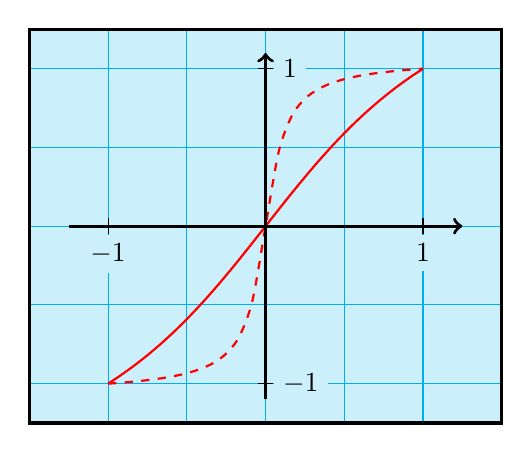
\begin{tikzpicture}
		% Hintergrund
		\fill[cyan!20] (-3, -2.5) rectangle (3, 2.5);
		\draw[thin, cyan, step=1] (-3, -2.5) grid (3, 2.5);

		% Funktionen
		\draw[thick, red] plot[smooth, domain=-2:2] (\x, {2*atan(\x/2)/atan(1)});
		\draw[thick, red, dashed] plot[smooth, domain=-2:2] (\x, {2*atan(5*\x)/atan(10)});

		% Achsen
		\draw[very thick, ->] (-2.5, 0) -- (2.5, 0);
		\draw[very thick, ->] (0, -2.2) -- (0, 2.2);
		\draw[thin] (-2, 0.1) -- (-2, -0.1) node[below, fill=cyan!20] {$-1$};
		\draw[thin] (2, 0.1) -- (2, -0.1) node[below, fill=cyan!20] {$1$};
		\draw[thin] (-0.1, -2) -- (0.1, -2) node[right, fill=cyan!20] {$-1$};
		\draw[thin] (-0.1, 2) -- (0.1, 2) node[right, fill=cyan!20] {$1$};

		% Rahmen
		\draw[very thick] (-3, -2.5) rectangle (3, 2.5);
	\end{tikzpicture}
	\caption{Graph for $u_1$ and $u_{10}$ from Weierstrass example.}
	\label{fig:example_1_3_1}
\end{figure}

The idea behind is that $u'$ should be more or less zero, and hence $u$ should be approximately piecewise constant. We compute
\[I(u_k)=\int_{-1}^1{x^2\left(\frac{\frac{1}{1+(kx)^2}\cdot k}{\arctan(k)}\right)^2\mathrm{d}x}=\frac{1}{\arctan(k)^2}\int_{-k}^k{\underbrace{y^2\frac{1}{1+y^2}}_{\leq1}\frac{\mathrm{d}y}{k}}\leq\frac{2}{\arctan(k)^2}\to0\]
for $k\to\infty$. So $(u_k)_{k\in\mathbb{N}}$ is an infimizing sequene. But we also claimed that there are no minimizers in $M$. This is true because if $u\in M$ then $I(u)>0$ since $I(u)=0$ would lead to $u'=0$ which is a contradiction to $u(-1)=-1$ and $u(1)=1$.\\

One can show that if $I(u)\ll1$ then $u|_{[0,1]}\approx1$ and $u|_{[-1,0]}\approx-1$, so a candidate for a minimizer is
\[u_*:[-1,1]\longrightarrow\mathbb{R},\qquad u_*(x):=\sgn{x}.\]
We will indeed show in the exercise lesson that every infimizing sequence $(u_k)_{k\in\mathbb{N}}$ of $I$ converges uniformly on any compact subset of $[-1,0)\cup(0,1]$ to $u_*$, i.e. $u_k\to u_*$ in $L_\text{loc}^\infty([-1,0)\cup(0,1])$. But $u_*$ does not belong to our class of functions we are considering. So the mathematical question is to find a space $\widetilde{X}\supset X$ such that $u_*\in\widetilde{X}$.
\end{example}

\begin{example}
Define the space of piecewise $C^1$-functions, i.e.
\[PC^1([a,b]):=\left\{u\in C^0([a,b])\,\middle\vert\,\exists a=x_0<x_1<\dotsc<x_n=b\text{ with }u|_{[x_{j-1},x_j]}\in C^1([x_{j-1},x_j])\right\}.\]
Now consider $X:=PC^1([0,1])$, $M:=\{u\in PC^1([0,1])\mid u(0)=0,u(1)=0\}$ with the functional
\[I:X\longrightarrow\mathbb{R},\qquad I(u):=\int_0^1{(1-(u'(x))^2)^2+u(x)^2\mathrm{d}x}.\]
We claim that $\inf_{u\in M}{I(u)}=0$, and to see this we are going to choose a sequence $(u_n)_{n\in\mathbb{N}}\subseteq M$ with the properties $\lvert u_n\rvert\leq\frac{1}{2n}$ and $u_n'\in\{-1,1\}$ for all $n\in\mathbb{N}$. A possible choice for such functions is illustrated in \hyperref[fig:example_1_3_3]{Figure I.6}.

\begin{figure}[h]
	\centering
	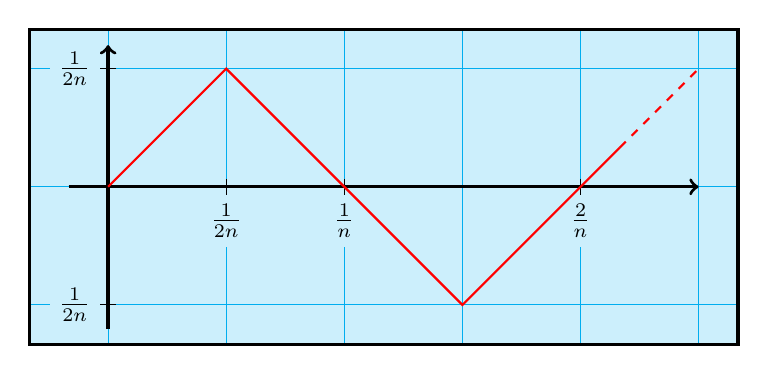
\begin{tikzpicture}
		% Hintergrund
		\fill[cyan!20] (-1, -2) rectangle (8, 2);
		\draw[thin, cyan, step=1.5] (-1, -2) grid (8, 2);

		% Achsen
		\draw[very thick, ->] (0, -1.8) -- (0, 1.8);
		\draw[very thick, ->] (-0.5, 0) -- (7.5, 0);
		\draw[thin] (1.5, 0.1) -- (1.5, -0.1) node[below, fill=cyan!20] {$\frac{1}{2n}$};
		\draw[thin] (3, 0.1) -- (3, -0.1) node[below, fill=cyan!20] {$\frac{1}{n}$};
		\draw[thin] (6, 0.1) -- (6, -0.1) node[below, fill=cyan!20] {$\frac{2}{n}$};
		\draw[thin] (0.1, -1.5) -- (-0.1, -1.5) node[left, fill=cyan!20] {$\frac{1}{2n}$};
		\draw[thin] (0.1, 1.5) -- (-0.1, 1.5) node[left, fill=cyan!20] {$\frac{1}{2n}$};

		% Funktion
		\draw[thick, red] (0, 0) -- (1.5, 1.5) -- (4.5, -1.5) -- (6.5, 0.5);
		\draw[thick, red, dashed] (6.5, 0.5) -- (7.5, 1.5);

		% Rahmen
		\draw[very thick] (-1, -2) rectangle (8, 2);
	\end{tikzpicture}
	\caption{Example for a function $u_n$ from Young's example.}
	\label{fig:example_1_3_3}
\end{figure}
With such a sequence we have
\[I(u_n)=\int_0^1{(1-u'_n(x)^2)^2+u_n(x)^2\mathrm{d}x}\leq\frac{1}{4n^2}\to0\]
as $n\to\infty$. Hence, $\inf_{u\in M}{I(u)}\geq0$. Moreover, it holds $u_n\to u_*$ in $C^0([0,1])$ uniformly, where $u_*\equiv0$. But $I(u_*)=1\ne0$.
\end{example}

\begin{remark}
\begin{itemize}
	\item[(a)] In \hyperlink{example_1_3_1}{Example 1.3.1} we saw that there exists a function which minimizes $I$, even if it does not lie in $M$.
	\item[(b)] In \hyperlink{example_1_3_2}{Example 1.3.2} something strange did happen. We constructed an infimizing sequence which actually converges uniformly in $C^0$ to the zero function, which even lies in $M$. So everything looks nice. But the zero function does not minimize our functional. The problem is that $I$ is not continuous with respect to uniform convergence.
\end{itemize}
\end{remark}